\section{Experimental Results}

\subsubsection{Two scenarios}
We illustrate dynamic aggregation with a common usage scenario.  Imagine there are a number of people in a building,
each owning a number of plug-load applicances and a laptop.  Assume that when a person is in a room their laptop
is plugged in and when they leave the room they unplug their laptop and take it with them.  People come and go
throughout the day, changing the aggregate power consumption of the room and it happens.  In addition, some
of those people move to other rooms and plug their laptop in the new location.  As this happens, we will assume
all actions are being recorded in StreamFS.

%FILL IN WITH REAL GRAPH
\begin{figure}[htb!]
\begin{center}
\subfloat[Room 1 object and aggregate streams.]{%
            \label{fig:dynaggs1room1}
            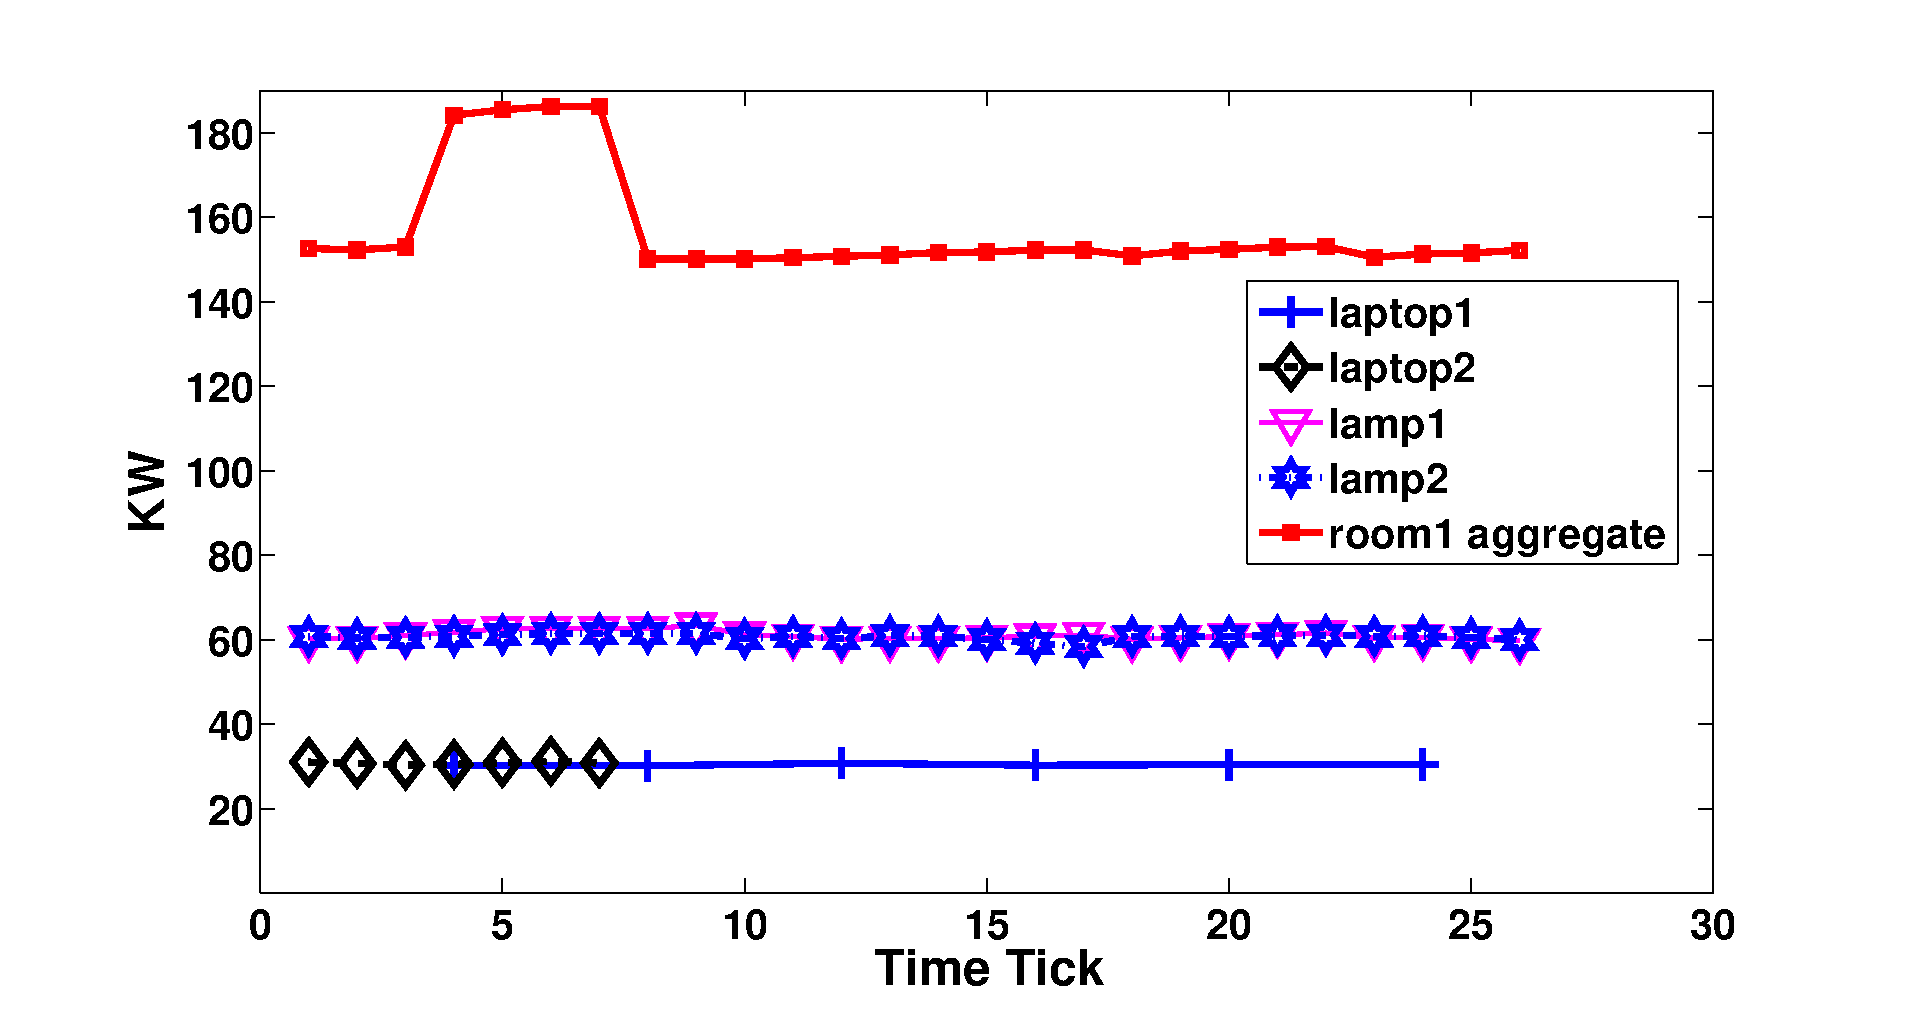
\includegraphics[scale=0.4]{figs/dynagg_scenario1_room1}
        }
\subfloat[Room 2 aggregate.]{%
            \label{fig:dynaggs1room2}
            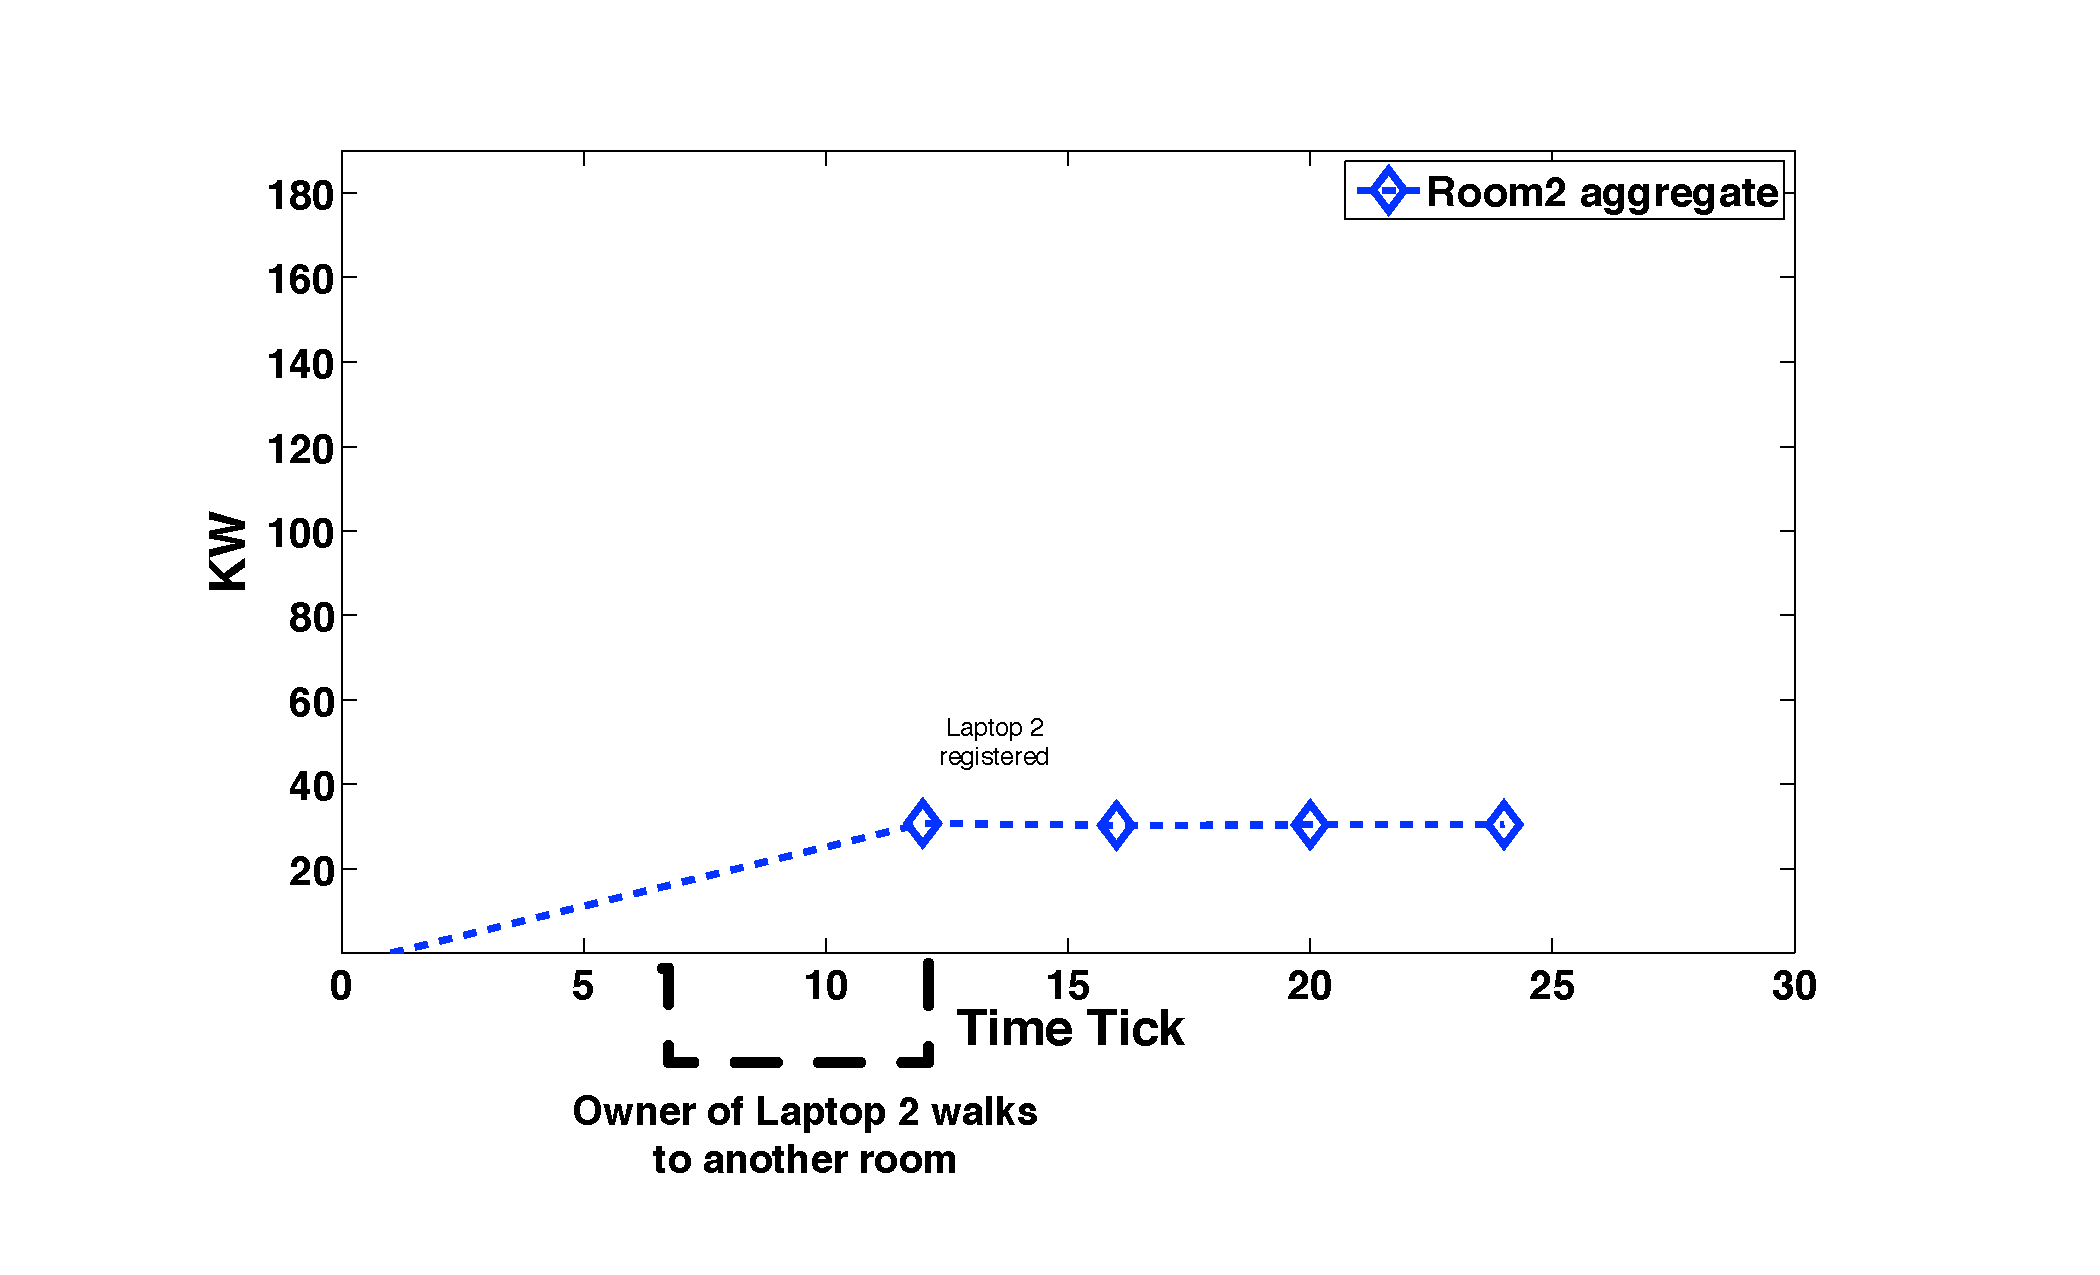
\includegraphics[scale=0.4]{figs/dynagg_scenario1_room2}
        }
\end{center}
\caption{
	The power consumes by a laptop in \emph{room 1} is shifted to \emph{room 2} a time t=7.  Notice the aggregagate drops in room 1
	while it rises in room 2.
     }%
\label{fig:multiroomagg}
\end{figure}

Figure~\ref{fig:multiroomagg} illustrate the aggregation results of that scenario.  Notice how...




\begin{figure}[t!] %htbp
\centering
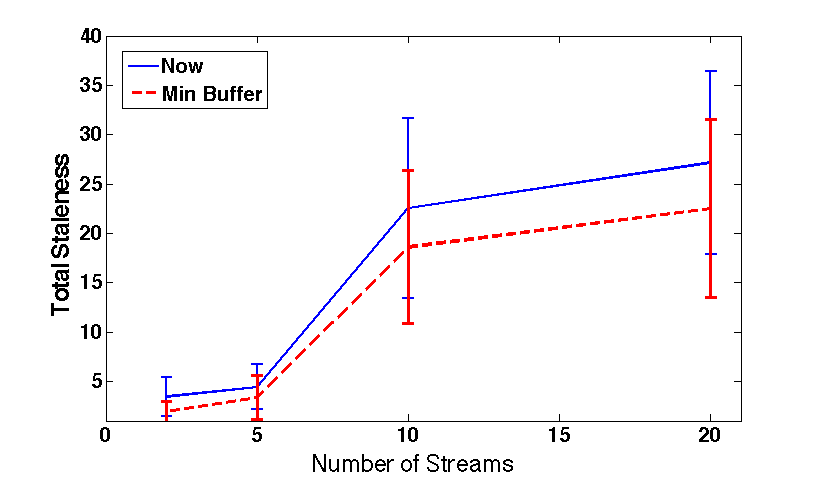
\includegraphics[width=0.9\columnwidth]{figs/staleness_vs_numstreams}
\caption{This figures shows the tradeoff between staleness and the number of streams being consumed by the job.  Note 
that out algorithm reduces the staleness of the buffer.}
\label{fig:stalevsstreams}
\end{figure}

\begin{figure}[t!] %htbp
\centering
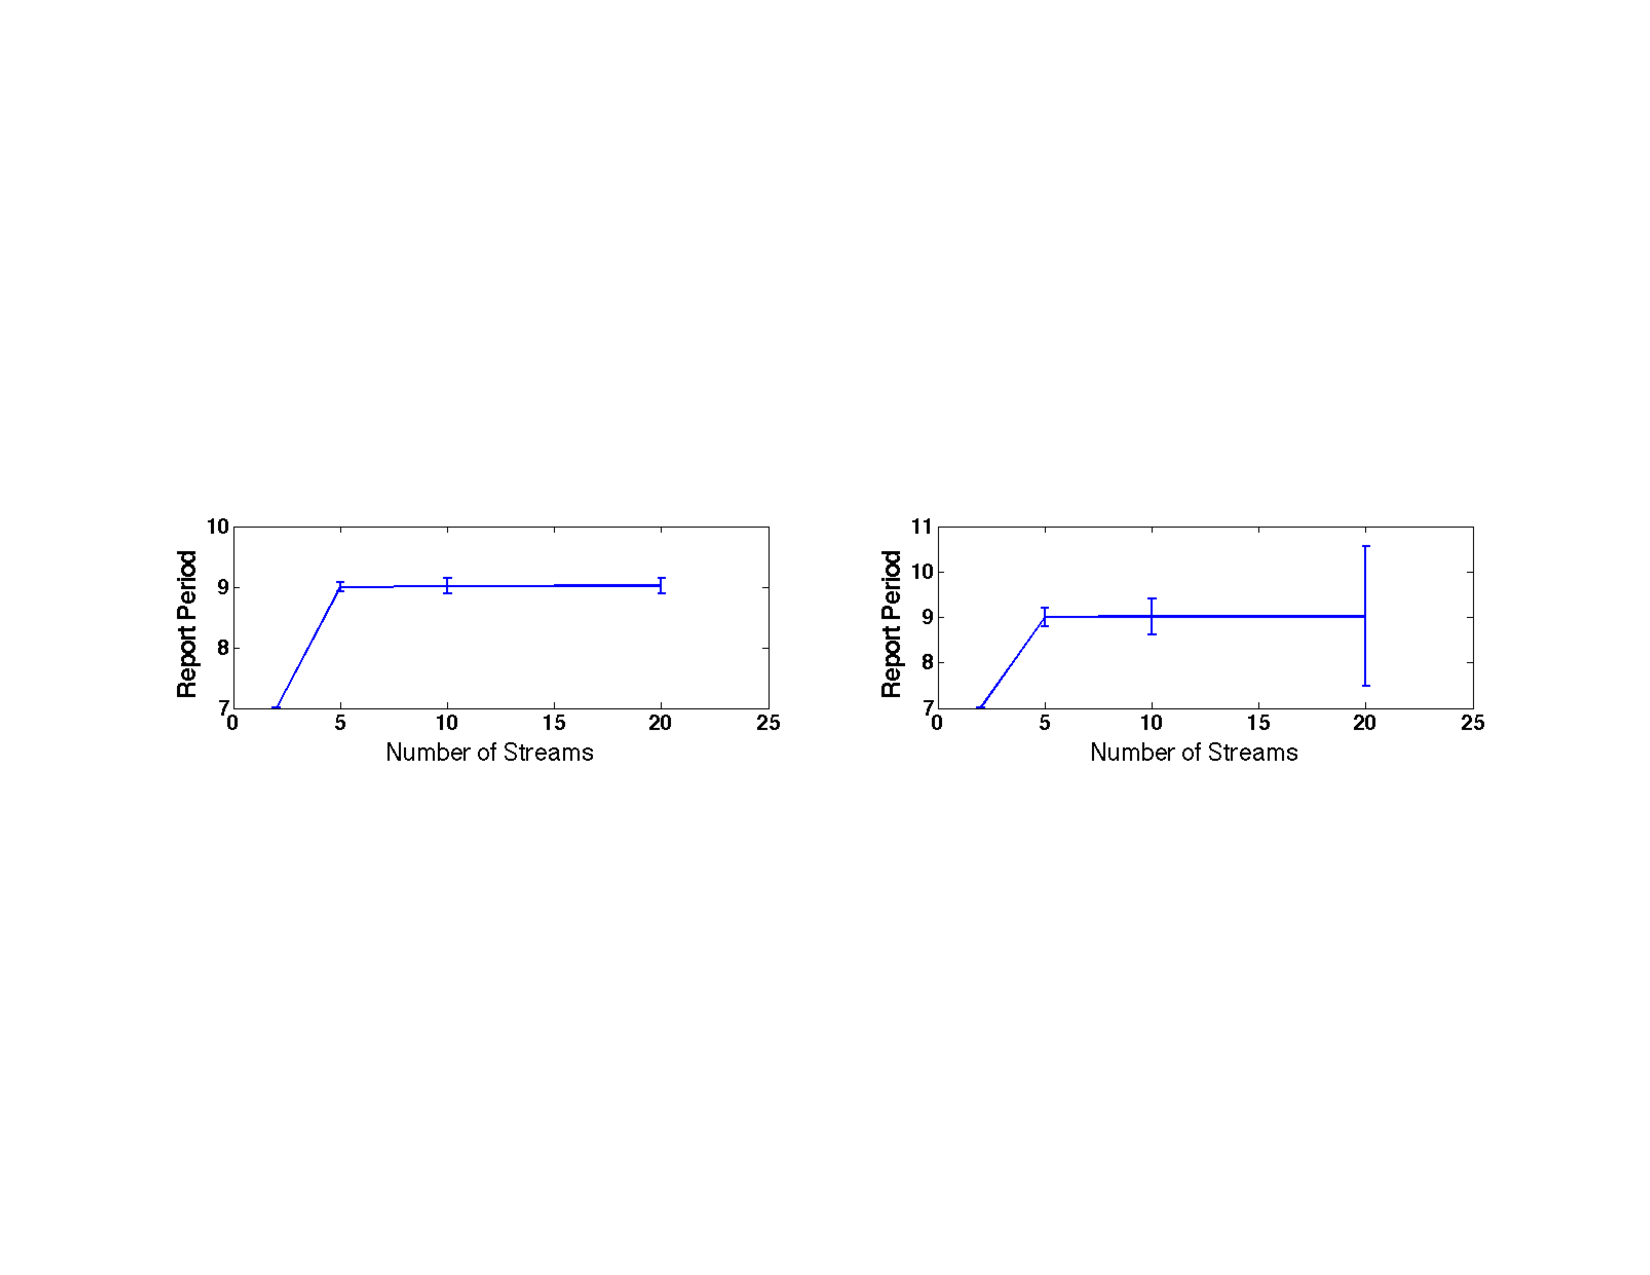
\includegraphics[width=1.0	\columnwidth]{figs/period_vs_streams}
\caption{This figures shows that the \texttt{min\_buffer} algorithm provides a similar average execution period but generally
at the cost of higher variance in delivery times.}
\label{fig:report_periods}
\end{figure}